\newpage
\thispagestyle{empty}

\chapter{Components}

\begin{figure}[H]
	\centering
	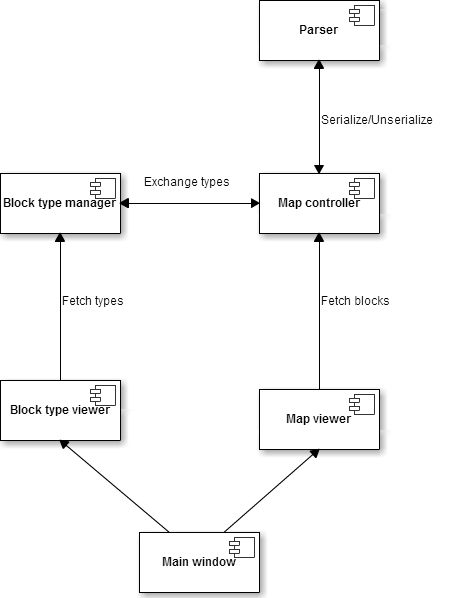
\includegraphics[scale=0.70]{component.png}
	\caption{Component diagram}
\end{figure}

\section{Parser}
The parser has two gaols, first load a map from JSON file, then write JSON file from existing map.
\section{Block type manager}
The block type manager manage every types of block and save them to the map controller. 
\section{Block type viewer}
The block type viewer will display the block types according to the block type manager and provide interections with it. It allows to create a new type, to edit or to delete an existing type.
\section{Map controller}
The map controller manage the map storage.
\section{Map viewer}
The map viewer will display the map according to the map controller and provide interections with it.
\section{Main window}
The main window provide interections between all the modules.